\section{Introduction}
\label{sec:introduction}
% state the learning objective 
The objective of this laboratory assignment is to simulate a AC/DC converter circuit, which output voltage must be ideally 12 Volts. 
This converter must have an envelope detector and a voltage regulator. We are free to choose the architecture of both circuits, 
however we must consider the cost of the components in the circuit, the ripple voltage and the voltage difference between the output 
voltage and 12 Volts.

After multiple simulations, we have decided to simulate the following circuit. The envelope detector is composed by
a full rectifier brigde and a resistor $R_1$ in parallel with a capacitor $C$, while the voltage regulator has a resistor $R_2$ in
series with 20 diodes. The values of the components are exhibited in the table below. We have also taken advantage of the fact that,
in this assignment, the number of turns $n$ of the transformer will not influence the merit of our work. Therefore, as you can see below,
we used an unusual value for $n$.


% COLOCAR DADOSIn order to analyse the circuit, the following data were obtained by running the supplied Python script

\par The voltage source is defined by:
\begin{equation}
v_s(t) = V_s u(-t) + sin(2 \pi f t)u(t)
\label {equation:voltsource}
\end{equation}
, where
\begin{equation}
u(t)=
\begin{cases}
0 & $t$ < $0$ \\
1 & $t $\geq$ 0$
\end{cases}
\label {eq:ut}
\end{equation}

In Section~\ref{sec:analysis}, a theoretical analysis of the circuit, 
performed on Octave, is presented. In Section~\ref{sec:simulation}, the 
circuit is analysed by simulation, using NGSpice, and the results are compared to 
the theoretical results obtained in Section~\ref{sec:analysis}. The conclusions 
of this study are outlined in Section~\ref{sec:conclusion}.

\begin{figure}[H] \centering
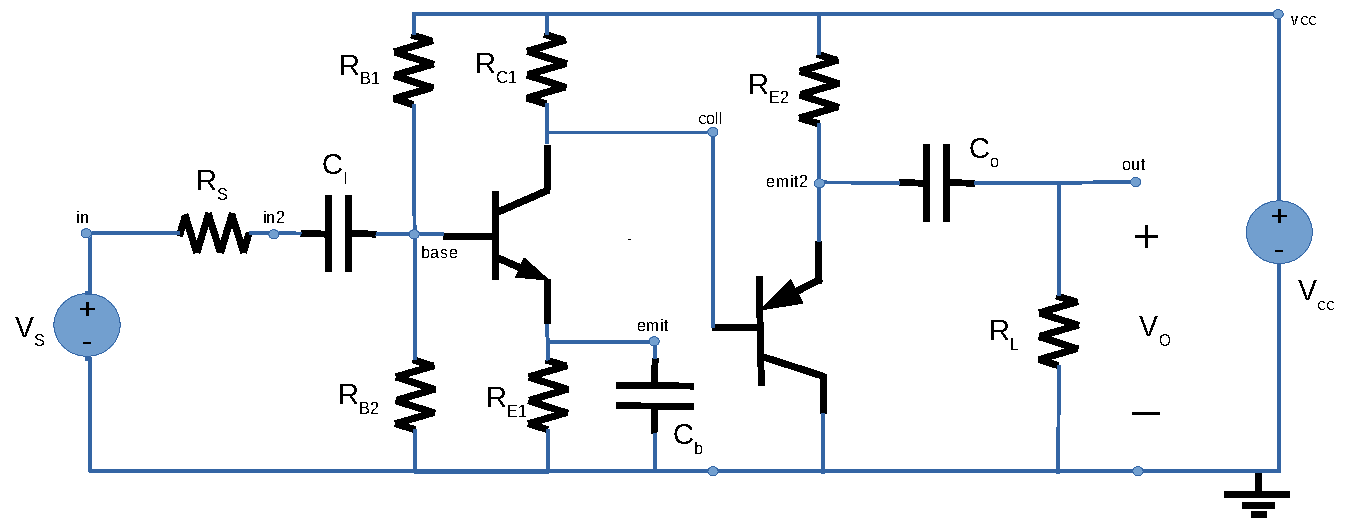
\includegraphics[width=0.4\linewidth]{circuit.pdf}
\caption{AC/DC converter circuit.}                                     %%%%%%%%%%LEGENDA
\label{fig:circuit}
\end{figure}

